\documentclass[conference]{IEEEtran}
\IEEEoverridecommandlockouts
% The preceding line is only needed to identify funding in the first footnote. If that is unneeded, please comment it out.
\usepackage{cite}
\usepackage{amsmath,amssymb,amsfonts}
\usepackage{algorithmic}
\usepackage{graphicx}
\usepackage{textcomp}
\usepackage{xcolor}
\usepackage[english]{babel}
\usepackage{booktabs} % For improved table formatting
\usepackage{array} % For improved column formatting
\usepackage{multicol} % For multi-column formatting
\usepackage{url}

\def\BibTeX{{\rm B\kern-.05em{\sc i\kern-.025em b}\kern-.08em
    T\kern-.1667em\lower.7ex\hbox{E}\kern-.125emX}}
\begin{document}

\title{Securing Data in Low-Resource Systems: Lightweight Block Cryptography Strategies}


\author{\IEEEauthorblockN{Fernando Ramirez Arredondo}
\IEEEauthorblockA{\textit{dept. name of organization (of Aff.)} \\
\textit{name of organization (of Aff.)}\\
Arequipa, Perú \\
fernando.ramirez@ucsp.edu.pe}
\and
\IEEEauthorblockN{Yván Jesús Túpac Valdivia}
\IEEEauthorblockA{\textit{dept. name of organization (of Aff.)} \\
\textit{name of organization (of Aff.)}\\
Arequipa, Perú \\
ytupac@ucsp.edu.pe}}


\maketitle

\begin{abstract}
    Secure communication for resource-constrained devices is crucial in today's world. This work classifies seven lightweight block ciphers designed for such devices. These ciphers offer efficient encryption for data security while minimizing resource consumption. Our analysis focuses on the two main categories of lightweight block ciphers, Substitution-Permutation Networks and Feistel Networks. We explore the key strategies these ciphers leverage within their chosen structures to achieve state-of-the-art performance. In particular, the analysis reveals that two prominent techniques are employed, bit-slicing and structure modification. These techniques play a significant role in optimizing the ciphers for resource-constrained environments.
\end{abstract}

\begin{IEEEkeywords}
iot, feistel, substitution-permutation, resource-constrained, lightweight, cryptography
\end{IEEEkeywords}

\section{Introduction}


The Internet of Things (IoT) has spawned an era of interconnected devices, generating vast amounts of data and transforming our interaction with the physical world. However, this interconnectedness presents a growing security challenge. As Thakor et al. \cite{IoT_1} categorize, IoT devices fall into two resource-based groups, resource-rich devices like servers, personal computers, and smartphones, and resource-constrained devices like sensor nodes, RFID tags, and actuators (Table \ref{table:crypto_devices}). Securing the sensitive data generated or transmitted by these resource-constrained devices becomes particularly challenging due to their limitations.

\begin{table}[ht]
    \centering
    \caption{Cryptographic Approaches on Different Devices}
    \begin{tabular}{ll}
        \toprule
        \textbf{Device} & \textbf{Cryptography} \\
        \midrule
        Servers, Desktops and Smartphones & Conventional Cryptography \\
        Embedded Systems and RFID & Lightweight Cryptography \\
        \bottomrule
    \end{tabular}
    \label{table:crypto_devices}
\end{table}

This challenge is further amplified by the evolution of IoT, which has transitioned from smaller networks to wide area networks, leading to a rapid growth in the number of interconnected devices. As IoT applications increase, a substantial amount of sensitive data is exchanged, raising concerns about privacy and security. Increased device interconnectivity further intensifies these concerns, potentially exposing new vulnerabilities with each additional device. In a landscape with billions of interconnected devices, even a single security flaw can be exploited on a massive scale.

Just as physical security measures like locks, safes, and opaque envelopes protect our valuables, cryptography serves as the digital equivalent, safeguarding the integrity and confidentiality of data in our online activities. This work aims to contribute to the application of cryptography for resource-constrained devices in the ever-expanding IoT landscape, where robust security solutions are essential to trust the activities and processes we reproduce or create from scratch in the digital world. 
Traditional cryptography, often computationally intensive, is impractical for these resource-constrained devices.  Lightweight cryptography emerges as a modern solution, specifically designed for devices with limitations in memory, processing power, and energy consumption. It prioritizes low computational complexity and a small memory footprint.

Ciphers are categorized into two primary classes, asymmetric and symmetric. While asymmetric ciphers offer enhanced security features, they necessitate greater computational resources and often incur higher implementation costs. Consequently, they are less suitable for resource-constrained devices. Among symmetric ciphers, block ciphers and stream ciphers are the most prevalent.\cite{NIST} This study focuses on block ciphers, delving into two fundamental structures employed in lightweight block ciphers, Feistel Networks and Substitution-Permutation Networks.

The Feistel Network (FN) stands as a fundamental structure in block cipher design. It offers a modular and efficient approach to encryption, employing multiple rounds of data processing. In each round, a half-block of data is processed using a round function, often incorporating non-linear substitutions and permutations. The output of this function is then combined with the other half-block using an XOR operation, creating a dependency between rounds that strengthens the overall security.\cite{FEISTEL}

The Substitution-Permutation Network (SPN) is another prominent block cipher structure. It relies on a series of substitution and permutation stages. Substitution boxes (S-boxes) replace data bits with new values, introducing non-linearity to confuse potential attackers. Permutation boxes (P-boxes) rearrange the data bits, making it challenging to discern the original data.\cite{heys1996substitution}

Both FN and SPN structures offer advantages in lightweight cryptography. FN structures are known for their modularity and ease of implementation, while SPN structures provide inherent parallelism, potentially leading to faster encryption/decryption on certain architectures.

This paper delves into a detailed exploration of FN and SPN structures in the context of lightweight cryptography. We will provide a comprehensive analysis of their design principles, operational workflows, and suitability for resource-constrained devices. See Table \ref{table:abbreviations} for the full list of abbreviations.

\begin{table}[ht]
    \centering
    \caption{Table of Abbreviations}
    \begin{tabular}{ll}
        \toprule
        \textbf{Abbreviation} & \textbf{Definition} \\
        \midrule
        ASIC & Application-Specific Integrated Circuit \\
        DULBC & Dynamic Ultra-Lightweight Block Cipher \\
        FN & Feistel Network \\
        FPGA & Field-Programmable Gate Array \\
        GE & Gate Equivalents \\
        IVLBC & InVolutive Lightweight Block Cipher \\
        IoT & Internet of Things \\
        KSA & Key Scheduling Algorithm \\
        LBC & Lightweight Block Cipher \\
        LBCCS & Lightweight Block encryption algorithm \\
        & based on Combined Chaotic System \\
        NIST & National Institute of Standards and Technology (USA) \\
        P-box & Permutation box \\
        RFID & Radio Frequency IDentification \\
        S-box & Substitution box \\
        SPN & Substitution-Permutation Network \\
        $f$ & Function \\
        XOR & eXclusive OR \\
        \bottomrule
    \end{tabular}
    \label{table:abbreviations}
\end{table}

\section{State of the art}

\begin{table*}[ht]
    \centering
    \caption{Lightweight Block Ciphers}
    \begin{tabular}{lllll} 
     \toprule
     Algorithm & Key size & Block size & Structure & N. of rounds \\ 
     \midrule
     DULBC (Yang et al., 2022) \cite{DULBC} & 80/128 & 64 & SPN & 25/30 \\
     GIFT (Yasmin and Gupta, 2023)\cite{GIFT}\cite{yasmin2023modified} & 128 & 64/128 & SPN & 28/40 \\
     IVLBC (Huang et al., 2023)\cite{IVLBC} & 80/128 & 64 & SPN & 29 \\
     LBC-IoT (Ramadan et al., 2021)\cite{LBC-IoT} & 80 & 32 & Feistel & 32 \\
     SAND (Chen et al., 2021)\cite{SAND} & 128 & 64/128 & Feistel & 48/54 \\
     LBCCS (Zhu et al., 2022)\cite{LBCCS} & 128 & 128 & Feistel & 20 \\
     SCENERY (Feng and Li et al., 2022)\cite{SCENERY} & 80 & 64 & Feistel & 28  \\
     \bottomrule
    \end{tabular}
    \label{table:ciphers}
\end{table*}

As shown in Table \ref{table:ciphers}, these algorithms are categorized based on their design principles. Each algorithm's performance is assessed considering factors like key size, block size, and the number of rounds employed during encryption. The rest of this section discusses the LBCs categorized by their underlying structure and mentions the main characteristics and approaches that give each cipher state of the art results.

\subsection{SPN-based solutions}

Yang et al. introduced DULBC, a dynamic SPN structure in which the specific encryption process changes based on the round keys. DULBC utilizes a unique approach where the round function isn't fixed. Each round selects one of four $f$ based on the first two bits of the round key, making it more resistant to attacks compared to static ciphers. This enhances security without significant hardware overhead. The proposed S-box offers good cryptographic properties with minimal logic gates, only 12 GEs. It consists of three NOR and XOR, one NAND and XNOR operations. leading to a simple inverse and efficient implementation. The authors highlight successful FPGA and ASIC implementations of DULBC, demonstrating its high throughput and relatively low area requirements. Security analysis confirms DULBC's resistance to various attacks, including differential attacks, linear attacks, and side-channel attacks. In conclusion, DULBC presents a promising solution for resource-limited environments due to its dynamic structure, efficient S-box design, and strong security profile.\cite{DULBC}


Yasmin and Gupta proposed a modification to the LBC GIFT. The main focus is on improving diffusion, how a single bit change in the message spreads throughout the ciphertext. It improves upon the original GIFT by enhancing the Key Scheduling Algorithm (KSA) using bit-slicing substitution and involutive permutation. By operating on multiple bits at once, in bit-slicing substitution, the larger data element (like a key) is sliced into smaller pieces. Each slice is then independently subjected to the substitution operation using the S-box. This allows for parallel processing of multiple bits simultaneously, taking advantage of the processor's architecture. By shuffling the bits and then applying the inverse permutation later, the original bit positions are obscured, making it harder to track how changes in the plaintext affect the ciphertext, leading to better diffusion and randomness in round keys. This addresses the predictability issue of the original KSA.\cite{GIFT}\cite{yasmin2023modified}


Huang et al. presented a new LBC named IVLBC specifically designed for unified encryption-decryption circuits in resource-limited environments. The design prioritizes high diffusion for strong encryption, involution (meaning components return to their original state after two applications), for efficient implementation, and flexibility in hardware and software. To achieve these goals, IVLBC utilizes a Feistel structure with a tree-based design for a compact and efficient S-box, by using a tree-based structure with logic operations, the S-box in IVLBC can achieve the same functionality as a traditional table-based S-box while requiring less memory and potentially faster processing. Additionally, it employs a unique nibble-based involutive permutation to enhance diffusion. Using nibble-based operations can further enhance diffusion by disrupting patterns across larger chunks of data compared to single-bit permutations. A significant advantage of IVLBC is that decryption can reuse the same circuitry as encryption, leading to lower resource requirements.\cite{IVLBC}

\subsection{FN-based solutions}

Feng and Li introduced a new LBC called SCENERY. To achieve low-cost hardware and efficient software implementation, they use bit-slicing techniques in the design of their f function. This means that each bit of the data block is processed in a separate, smaller unit called a slice, rather than working with entire blocks. The main benefits of this implementation are speed improvements on hardware that supports parallel execution and simpler logic circuits in hardware design, potentially reducing area and power consumption compared to traditional designs. While bit-slicing increases code complexity, lightweight ciphers are not complex by definition, so this is not a significant issue.
To address the slow diffusion issue that can occur with a balanced Feistel structure, SCENERY incorporates a 32x32 binary matrix that can be implemented efficiently and improves diffusion speed. The paper also proposes a new KSA to tackle the issue of backward derivation of the master key. While not a complete solution, this method makes it more difficult compared to PRESENT's key scheduling\cite{PRESENT} and enhances the security of key expansion.\cite{SCENERY}


LBCSS is a LBC that leverages a combined chaotic system for its design. This means that instead of relying on a single mathematical function that exhibit chaotic behavior, LBCSS uses multiple functions together. This chaotic system is used to create secure S-boxes, P-boxes, and keys for the encryption process. In terms of design specifics, LBCSS adopts a structure that enhances diffusion compared to the traditional generalized Feistel structure, but maintains a concise design. The cipher employs a non-linear round function created using a bit-slicing technique, this means the function introduces non-linear transformations on the data using operations like substitutions, rotations, or bitwise operations. These operations ensure a complex relationship between the original data and the encrypted output. This round function remains consistent across all encryption rounds to maintain low complexity. To prevent these consistent rounds from becoming too predictable, round constants are introduced to add variation. The authors argue that LBCSS offers sufficient security based on various tests, including resistance to different cryptanalysis methods and statistical testing.\cite{LBCCS}


Chen et al. proposed a new LBC named SAND. The main characteristic of this cipher is that it employs AND, Rotation, and XOR operations (AND-RX) within a Feistel structure. SAND allows for easier security evaluation compared to other AND-RX ciphers. Traditionally, evaluating the security of AND-RX ciphers can be complex because these operations often work on individual bits within the data, making it difficult to apply existing analysis methods typically used for S-boxes. This improvement is achieved by SAND utilizing AND-RX operations within small data units (nibbles). By working with nibbles instead of individual bits, SAND makes its security analysis easier. This allows security researchers to use existing methods designed for analyzing S-boxes, which are a more familiar and well-studied component in cryptography. The authors highlight the benefits of SAND in terms of both security and performance. SAND achieves strong security under various attack scenarios, including differential and linear attacks. The paper also discusses the motivations behind the design of SAND. Existing solutions for ARX-based ciphers often rely on large S-boxes, which are not ideal for hardware implementation. SAND aims to bridge this gap by providing an AND-RX design with efficient hardware implementation and strong security guarantees through its novel S-box transformation approach.\cite{SAND}


LBC-IoT incorporates two important cryptographic concepts, confusion and diffusion. Confusion scrambles the relationship between the original data and the encrypted data, while diffusion distributes the influence of a single bit change across the entire encrypted message. LBC-IoT achieves this by employing a combination of techniques, including a compact S-box with high non-linearity properties for data substitution and dedicated P-boxes for bit permutation, further obfuscating the relationship between the original and encrypted data. It is well known that FN structures can lack diffusion due to the round function $f$ being applied to only half of the data each round. LCB-IoT's solution to this problem is to apply a different P-box to each half of the data at the end of the rounds. The cipher utilizes simple operations within its core function and keeps the S-box size small. This approach minimizes the amount of processing power and memory required for implementation. Security-wise, LBC-IoT is resistant to brute-force attacks by adhering to NIST recommendations for key length. It uses an 80-bit key, which is too complex to crack through exhaustive searching methods. In essence, LBC-IoT offers a good balance between robust security and efficient implementation.\cite{LBC-IoT}

\section{Techniques to implement} \label{tecnicas}
In this section, we explore two cryptographic techniques commonly used for secure data encryption, Substitution-Permutation Networks and Feistel Networks. The focus of this section is to describe their structure, encryption process, decryption process and properties.\cite{zhong2024lightweight}
\begin{table}[ht]
    \centering
    \caption{Notations of Substitution-Permutation Network}
    \begin{tabular}{ll}
        \toprule
        \textbf{Notatios} & \textbf{Descriptions} \\
        \midrule
        $P$ & Plaintext \\
        $C$ & Ciphertext \\
        $K$ & Key \\
        $S_i$ & Substitution Box (S-box) \\
        $P$ & Permutation Box (P-box) \\
        $F$ & Round Function \\
        $\oplus$ & Bitwise XOR operation \\
        \bottomrule
    \end{tabular}
    \label{table:spn}
\end{table}

\begin{figure*}
    \centering
    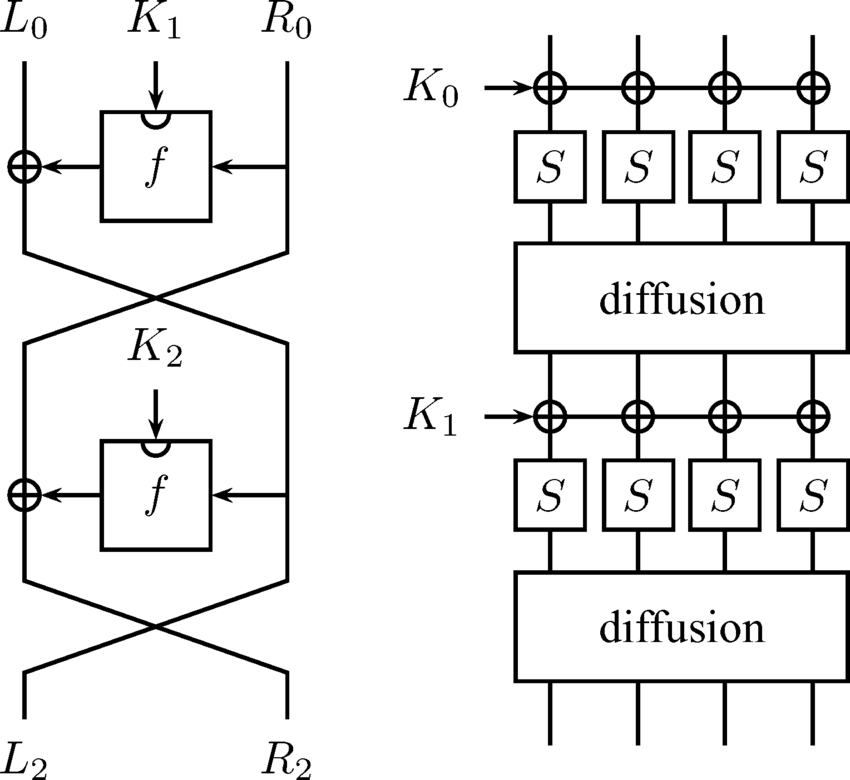
\includegraphics[width=\columnwidth]{figures/FEISTEL-SPN.png}
    \caption{Representation of a Feistel Network (left) and a Substitution-Permutation Network (right).}
    \label{fig:FEISTEL-SPN}
\end{figure*}

\subsection{Substitution-Permutation Network}
A Substitution-Permutation Network is a widely used design paradigm for block ciphers. It iterates a series of rounds, each consisting of two primary functions.
Refer to Fig. \ref{fig:FEISTEL-SPN} for a representation of a standard SPN and its components, including S (S-box), diffusion (P-box), and the corresponding subkey $K_n$ for $n$ representing each round.
\subsubsection{Substitution (S-boxes)}
These non-linear operations replace individual bits or groups of bits in the data block with new values, introducing confusion into the encryption process.
\subsubsection{Permutation (P-boxes)}
These functions rearrange the bits within the data block, achieving diffusion by spreading the influence of a single bit change across the entire ciphertext.
\subsubsection{Structure}

The SPN iterates these operations over multiple rounds, controlled by a round function $F$.
\subsubsection{Encryption Process (per round)}

Let $P_i$ be the i-th plaintext block and $K_i$ be the i-th round key derived from the main key K. The encryption process for a single round can be described as follows.

Substitution: Apply S-boxes to each sub-block of the data, where j iterates over the S-boxes and $\oplus$ denotes the bitwise XOR operation. 
\begin{align*}
    S_j(P_i \oplus K_i) \\
\end{align*}
Permutation: Permute the output of the S-boxes using the P-box.
\begin{align*}
    P(S_j(P_i \oplus K_i)) \\
\end{align*}
Output: The output of the P-box becomes the input for the next round or the final ciphertext if it's the last round.
This process is repeated for a specific number of rounds.
\subsubsection{Decryption}

Decryption essentially reverses the encryption process using the same SPN structure but with different round keys. The round keys are typically derived from the main key in a specific order, with the last round key used for decryption being the first round key for encryption and so on.
Let $C_i$ be the i-th ciphertext block and $K_i$ the round key for decryption, derived from K. The decryption process for a single round can be described as follows.

Inverse Permutation: Apply the inverse of the P-box.
\begin{align*}
    P^{-1}(C_i) \\
\end{align*}
Inverse Substitution: Apply the inverses of the S-boxes.
\begin{align*}
    S_j^{-1}(P^{-1}(CT_i) \oplus K_i') \\
\end{align*}
Output: The output of the inverse S-boxes becomes the input for the next decryption round or the final plaintext if it's the last round.
Similar to encryption, decryption is repeated for the specified number of rounds.
\subsubsection{Properties}
SPNs are a popular design choice for block ciphers due to their ability to achieve several key security properties.  SPNs achieve confusion by employing S-boxes that perform non-linear operations on the data, making the link between plaintext, key, and ciphertext highly complex. Additionally, P-boxes ensure diffusion by rearranging the data bits, such that a single change in the plaintext has a cascading effect on the final ciphertext. This characteristic, along with the avalanche effect (where minor variations in the plaintext or key lead to significant alterations in the ciphertext), helps resist attacks like differential cryptanalysis. Ultimately, the number of encryption rounds and the design of the S-boxes and P-boxes play a critical role in determining the overall strength and security of an SPN cipher.

\begin{table}[ht]
    \centering
    \caption{Notations of Feistel Network}
    \begin{tabular}{ll}
        \toprule
        \textbf{Notatios} & \textbf{Descriptions} \\
        \midrule
        $F$ & Feistel function \\
        $L_n, R_n$ & Left and right halves of the data block at round $n$ \\
        $L_{n+1}, R_{n+1}$ & Left and right halves of the data block after round $n$ \\
        $K_n$ & Round key for round $n$ \\
        $\oplus$ & Bitwise XOR operation \\
        \bottomrule
    \end{tabular}
    \label{table:fn}
\end{table}

\subsection{Feistel Network}
Feistel network, also known as a Feistel cipher, is a fundamental concept in cryptography. It's not a specific encryption algorithm itself, but rather a design framework used to build many powerful block ciphers. Refer to Fig \ref{fig:FEISTEL-SPN} for a representation of a standard FN and its round functions, denoted as $f$, receiving the data block $R_n$, representing the rightmost part of the full input, and the subkey $K_n$ for $n$ representing each round. $L_n$ represents the left part of the input.
\subsubsection{Structure}
A FN iterates a basic function, the Feistel function $F$, on the halves of the data block $(L_n, R_n)$ during each round.
\subsubsection{Encryption Process (per round)}
The network performs the following operations at each round $n$:
\begin{align*}
    L_{n+1} &= R_n \\
    R_{n+1} &= L_n \oplus F(R_n, K_n) \\
\end{align*}
where $K_n$ is a round key. After the final round, the outputs are swapped to obtain the ciphertext $(C_1, C_2)$.
\subsubsection{Decryption}
The decryption process in a FN is very similar to encryption, but the round keys are applied in reverse order. This allows the network to reverse the operations performed during encryption and recover the original data.
\subsubsection{Properties}
FNs boast several advantages for secure encryption. Each added round enhances the cipher's theoretical resistance to attacks. Under specific assumptions, their security can be mathematically proven based on the underlying Feistel function's strength. Additionally, the design offers flexibility by allowing customization of both the Feistel function and the number of rounds to achieve desired security levels. However, these networks also have drawbacks. The overall security hinges heavily on a strong Feistel function, and each round introduces processing overhead, potentially slowing down encryption and decryption.


\section{Conclusions}
Feistel Networks and Substitution-Permutation Networks are both fundamental structures for designing lightweight block ciphers. While they share some similarities, they have distinct advantages and disadvantages.

Feistel networks offer inherent invertibility, meaning decryption is straightforward even if the round function itself isn't invertible. This simplifies design and analysis.

Substitution-Permutation Networks can potentially achieve higher throughput due to their inherent parallelism, making them attractive for hardware implementations with multiple processing units.

The best choice between a Feistel Network and a Substitution-Permutation Network depends on the specific application and design goals. If ease of decryption and hardware limitations are key concerns, a Feistel Network might be preferable. If maximizing encryption speed on parallel hardware is a priority, a Substitution-Permutation Network might be a better choice.

Additionally, both Feistel Networks and SPNs can be further enhanced with techniques like bit-slicing, custom S-boxes, combined chaotic systems, and even including modifications to the underlying structure to improve security, performance, or both.

Bit-slicing allows for parallel processing on hardware that supports it, potentially leading to significant speed improvements. It's particularly beneficial for lightweight ciphers designed for resource-constrained environments. However, bit-slicing can increase code complexity, so it's important to find a balance between efficiency and implementation effort.
Some S-boxes might be designed with a low logic gate count for compact hardware implementations, while others might prioritize high non-linearity for enhanced security.
Some LBCs utilize combined chaotic systems together to enhance the complexity and randomness of the encryption process. This can be a promising approach for achieving strong security.

The development of lightweight cryptography seems to be a continuing search for balance between security and efficiency. On one hand, lightweight ciphers need to be strong enough to resist attacks, but on the other hand, they must also be efficient in terms of resource consumption (memory, processing power) to run on devices with limited capabilities.


\bibliographystyle{IEEEtran}
\bibliography{bibliography/references}
\vspace{12pt}


\end{document}
